\documentclass[12pt]{article}
\usepackage{fullpage} 
\usepackage{microtype}      % microtypography
\usepackage{array}
\usepackage{amsmath,amssymb,amsfonts}
\usepackage{amsthm}
\usepackage{graphicx}

%% Header
\usepackage{fancyhdr}
\fancyhf{}
\fancyhead[C]{CS 136 - 2022s - Checkpoint 2}
\fancyfoot[C]{\thepage} % page number
\renewcommand\headrulewidth{0pt}
\pagestyle{fancy}

\usepackage[headsep=0.5cm,headheight=2cm]{geometry}

%% Hyperlinks always blue, no weird boxes
\usepackage[hyphens]{url}
\usepackage[colorlinks=true,allcolors=black,pdfborder={0 0 0}]{hyperref}

%%% Doc layout
\usepackage{parskip}
\usepackage{times}

%%% Write out problem statements in blue, solutions in black
\usepackage{color}
\newcommand{\officialdirections}[1]{{\color{blue} #1}}

%%% Avoid automatic section numbers (we'll provide our own)
\setcounter{secnumdepth}{0}

\begin{document}
~~\\ %% add vert space

\begin{center}
{\Large{\bf Student Names: Nate Davis and Alexander Lobo}}
\end{center}

{\Large{\bf Collaboration Statement:}}

Turning in this assignment indicates you have abided by the course Collaboration Policy:

\url{www.cs.tufts.edu/comp/136/2022s/index.html#collaboration-policy}

Total hours spent: 10-15

We consulted the following resources:
\begin{itemize}
\item TODO
\item TODO
\item $\ldots$	
\end{itemize}

\newpage

These are the official instructions for checkpoint 2.  You can find instructions on how to submit at \url{www.cs.tufts.edu/comp/136/2022s/checkpoint2.html}

\textbf{Please consult the full project description at \url{https://www.cs.tufts.edu/comp/136/2022s/project.html} in addition to this document when working on this checkpoint.  It gives details on what we expect.}

\section{Applying Model to Dataset}

For this project, we have decided to implement a Bayesian Logistic regression model to predict the class of conformations of molecules as either "musk" or "non-musk".

We used the \texttt{MAPEstimator.py} class from CP2 as a template to set up our model. In our python file, we have a \texttt{MAPEstimator} class with an initialization (\texttt{\_init\_}). Various methods (\texttt{fit()}, \texttt{predict\_proba()}, and \texttt{score()}) are also implemented to train and test the model. Details of our implementation are below.

\subsection{Initialization}

The \texttt{MAPEstimator} class has the following attributes that are defined in the initialization:

\begin{itemize}
\item \texttt{w\_D} : defines the first instance of the weight vector

	\begin{itemize}
	\item is a vector of all zeros since our prior (both trivial and SAS) assumes a zero mean
	\end{itemize}
	
\item \texttt{prior} : determines which prior to use (\texttt{'trivial'} or \texttt{'sas'})

	\begin{itemize}
	\item \texttt{'trivial'} prior :
\begin{equation}
p(\textbf{w}|\alpha) = \mathcal{N}(\vec{0}, 	\alpha^{-1}I_{166})
\end{equation}
	\item \texttt{'sas'} prior (sas stands for "spike-and-slab" \footnote{\url{https://en.wikipedia.org/wiki/Spike-and-slab_regression}}):
\begin{equation}
p(\textbf{w}|\alpha,\beta) = 0.8\mathcal{N}(\vec{0}, 	\alpha^{-1}I_{166}) + 0.2\mathcal{N}(\vec{0}, 	\beta^{-1}I_{166})
\end{equation}
	\end{itemize}

\item \texttt{alpha} : A real value that determines the precision of either the trivial prior or first MVN in the SAS prior

\item \texttt{beta} : A real value that determines the precision of the second MV in the SAS prior (should only be specified if \texttt{prior='sas'}

\item \texttt{max\_iter} : A positive integer that determines the maximum number of iterations allowed for the stochastic gradient descent

\item \texttt{tol} : A real positive value that determines the tolerance for convergence for the stochastic gradient descent

\item \texttt{step\_size} : A positive real value that determine how large the weight update is per iteration

\end{itemize}

\subsection{Training}

The \texttt{fit()} method is used to train the Bayesian logistic regression model with the provided training data. Since stochastic gradient descent is being used, a while loop iterates over each training example to compute the gradient of the posterior distribution. This gradient is then used to update to update the weight vector and bias term according to the following equations, where $c$ is the bias term:

\begin{equation}
\mathbf{w}^{t+1} \leftarrow \mathbf{w}^{t} - \eta \left[ \left(\sigma(\mathbf{w}^t \cdot x^{(i)}) - y^{(i)}\right) x^{(i)} + \alpha \mathbf{w}^{t} \right]
\end{equation}

\begin{equation}
c^{t+1} \leftarrow c^{t} - \eta (\sigma(\mathbf{w}^t \cdot x^{(i)}) - y^{(i)})
\end{equation}

After each update, the log loss for that example is computed using the following equation:

\begin{equation}
L = y^{(i)} \log \hat{y}^{(i)}+ (1-y^{(i)})\log(1-\hat{y}^{(i)})
\end{equation}

This loss is then appended to a vector of losses. Since stochastic gradient descent is prone to fluctuations in the loss at each step, after 10 iterations, the previous ten losses are averages and then compared to the 10 before that to see if the average loss change is reducing. If the average loss change becomes less than the tolerance, then it is said to have converged and the loop halts. If the average change in loss does not converge, then the loop halts when the maximum number of iterations are reached.

\subsection{Evaluation}

The \texttt{predict\_proba()} method is used to predict the probability of each example being in the "musk" and "non-musk" class while the \texttt{score()} method uses a threshold of 0.5 to characterize each example and then compute the accuracy of the predictions by comparing to the true class labels. After splitting our data set into a training and testing set and training the model on the training set, we can evaluate the models performance by calculating the prediction score with the testing set. We can also use the \texttt{iter\_count} attribute to evaluate many iterations it took for the training to converge.

\subsection{Bottlenecks}

We decided to first test our model with a learning rate and $\alpha$ value of both 1. However, upon implementation, we noticed that the model would not converge, instead, the loss would shoot up to infinity after a few iterations. We then normalized the data using a standard scaler, assuming that the large feature values were causing large steps in the weight updates. However, this led to the same result. After deliberating, we decided to reduce our step-size to 0.001. After this change, the average loss started decreasing with each iteration and took on average about 100 iterations to converge with an average testing accuracy of 75\%.***

***Need to update this once we finalize our testing


\section{Evaluating Hypotheses from Checkpoint 1}

We have tweaked our hypotheses from Checkpoint 1. The one that is testable at this stage is now:

\begin{itemize}
    \item We hypothesize that our multivariate logistic regression model with first-order stochastic gradient descent will converge in fewer iterations, but with ultimately similar accuracy, when we use different step sizes for misclassifying the two output classes, as our output classes are highly imbalanced.
\end{itemize}

We evaluated this hypothesis via (shuffled) K-fold cross validation with 10 folds, noting how many iterations it took the model to converge for each fold and the accuracy on the held-out examples. The hyperparameters held fixed across the tests were a prior weight vector of zeros with precision of 0.1, a standard step size of 0.1 and, in the dynamic case, a step size of 0.2 for musks, a convergence tolerance of $10^{-4}$, and a max iteration count of 10,000,000.

The results can be seen in the following graphs:

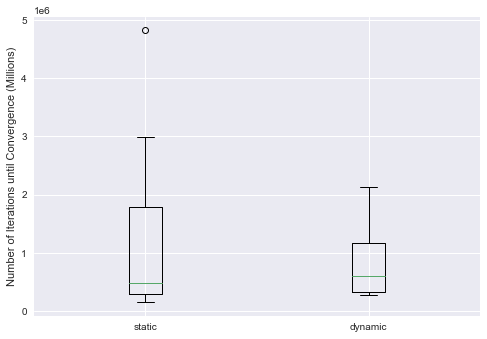
\includegraphics[scale=.7]{iter_counts.png}

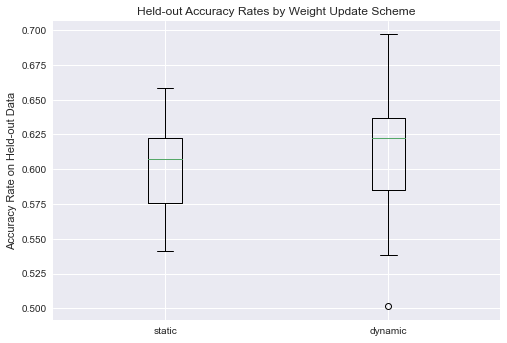
\includegraphics[scale=.7]{accuracy_rates.png}

The first shows the distribution of iteration counts (in millions) for the training of each of the models until convergence. The median of the model trained with dynamic step size is slightly higher than that of the static model, but the variance is much smaller, especially on the high end. The longest the dynamic model took to train was approximately 2 million iterations while the static model has two training runs that took far longer. The interquartile range for the model with dynamic step size is also quite a bit smaller.

As for accuracy rate, the results are somewhat flipped, with the dynamic step size model having a higher median and interquartile range, but a much larger range of outcomes overall. 

Our hypothesis, which contains two sub-hypotheses, was correct to an extent. The model with dynamic step size certainly seems to have iteration counts that generally cluster around a lower value, but the median value for the static step size is actually smaller. The difference really seems to be more about variance than a representative value.

As for the accuracy rate, we did not foresee the dynamic model performing better than the static, and also said nothing regarding the variance of results. We thought that the models might converge to the same places, but perhaps with the randomness we introduced into the training process, the models reached our (somewhat arbitrary) conversion threshold at different times.


\section{Proposing an Upgrade to your Model or Learning Method}

The purpose of this study is to explore how our model performs when upgrading our
learning method from a first order to a second order gradient descent algorithm to solve the
weight vector MAP estimate for logistic regression. We propose the following hypotheses
for how we expect our model to perform:

\end{document}


